\section{Penalized maximizers are almost balanced}\label{sec:variations}

A maximum polygon cap is balanced \baek{Thm.~3.4.9}: $\sigma_K(t)=\tau_K(t)$ for
every $t\in\Theta^\diamond$, since otherwise pushing one side would increase
$\cA_\Theta$. A penalized maximizer need not be balanced, but pushing a side
changes the penalty by a controlled amount, and the argument gives a one-sided
bound on the \emph{defect}
\[
  \zeta_K(t)=\sigma_K(t)-\tau_K(t).
\]
In this section we fix $k\ge0$, $\Theta=\Theta_k$, a penalized maximizer
$K\in\Kc_k$ at stage $k$, and $\eta\ge0$ with $\abs{h_K(s)-h_*(s)}\le\eta$ at
every sampled normal $s$. Let
\[
  \bar\nu=\sum_s\nu_k(s)
\]
be the total weight; $\bar\nu\le1$ by \eqref{eq:weights}.

\begin{figure}[ht]
\centering
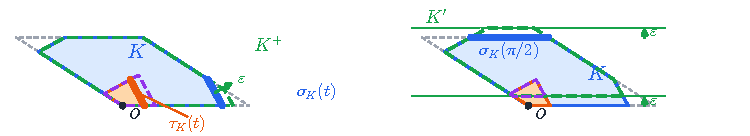
\includegraphics[width=\linewidth]{figures/fig-moves}
\caption{Pushing one side of a polygon cap $K$ with angle set $\{\omega/2\}$,
$\omega=1$; the grey dashed parallelogram is $P_\omega$, and the niche of $K$ is
orange. Left: raising the height at the floating normal $t=\omega/2$ by $\eps$
gives the cap $K^+$ (green, dashed) and its niche (purple, dashed); the cap
gains a strip of area $\sigma_K(t)\eps+O(\eps^2)$ along its edge with normal
$t$, and the niche a strip of area $\tau_K(t)\eps+O(\eps^2)$ along the side on
the inner wall $b_K(t)$. Right: raising the pinned height at $\pi/2$ by $\eps$
moves both lines of the horizontal strip up by $\eps$ (green, dotted) and gives
$K'$ (green, dashed), with its niche (purple, dashed); the cap gains a strip
along its top edge, of length $\sigma_K(\pi/2)$, and loses one along its bottom
edge, and $K'$ is a translate of a polygon cap.}
\label{fig:moves}
\end{figure}

\subsection{Floating normals}

\begin{lemma}[raising a floating height]\label{lem:floating}
Let $K\in\Kc_\Theta$, $t\in\Theta^\diamond\setminus\{\omega,\pi/2\}$,
$\eps\ge0$, and $K^+=\cC_\Theta(h_K^{t,\eps})$. Then $K^+\in\Kc_\Theta$,
$K\subset K^+$, and
\[
  h_{K^+}(s)=h_K(s)\quad\text{for }s\in\Theta^\diamond\setminus\{t\},\qquad
  h_K(t)\le h_{K^+}(t)\le h_K(t)+\eps.
\]
\end{lemma}

\begin{proof}
Since $h_K(\omega)=h_K(\pi/2)=1$, $P_{h^{t,\eps}_K}=P_\omega$, so
\[
  K^+=P_\omega\cap\bigcap_sH_-\bigl(s,h^{t,\eps}_K(s)\bigr),
\]
the intersection over the floating normals $s$. As $h_K\le h^{t,\eps}_K$,
\[
  K=\cC_\Theta(h_K)\subset K^+\subset P_\omega.
\]
So $K^+$ is a convex body (it is bounded, since the half-planes with normals
$t'$ and $t'+\pi/2$, $t'\in\Theta$, bound it also when $\omega=\pi/2$), it has
the support values $1,1,0,0$ of $P_\omega$ at $\omega,\pi/2,\omega+\pi,3\pi/2$,
and it is an intersection of half-planes with the normal angles of a polygon
cap. So $K^+\in\Kc_\Theta$. Next, $h_{K^+}\ge h_K$ since $K\subset K^+$, and
$h_{K^+}(s)\le h_K^{t,\eps}(s)$ since $K^+\subset H_-(s,h^{t,\eps}_K(s))$.
\end{proof}

\begin{proposition}[floating defects]\label{prop:floating}
For every floating normal $t\in\Theta^\diamond\setminus\{\omega,\pi/2\}$,
\[
  \sigma_K(t)-\tau_K(t)\le2\eta\,\nu_k(t).
\]
\end{proposition}

\begin{proof}
Let $K^+_\eps=\cC_\Theta(h^{t,\eps}_K)$. By \cref{lem:floating}, $K^+_\eps$ is a
polygon cap that has the support values of $K$ on
$\Theta^\diamond\setminus\{t\}$, and differs from $K$ at $t$ by at most $\eps$;
so by \eqref{eq:penalty-change-one},
\[
  \Pi_k(K^+_\eps)-\Pi_k(K)\le\nu_k(t)(2\eta\eps+\eps^2).
\]
Penalized maximality gives
$\cA_\Theta(K^+_\eps)-\cA_\Theta(K)\le\Pi_k(K^+_\eps)-\Pi_k(K)$. By
\cref{fact:push}\ref{fact:push:area} (with $C=K^+_\eps$, $v=0$) and
\ref{fact:push:derivative}, for small $\eps$
\[
  \cA_\Theta(K^+_\eps)\ge\cA_\Theta(h_K^{t,\eps})\ge\cA_\Theta(K)+(\sigma_K(t)
    -\tau_K(t))\eps-M\eps^2 .
\]
Hence
\[
  (\sigma_K(t)-\tau_K(t))\eps-M\eps^2\le\nu_k(t)(2\eta\eps+\eps^2).
\]
Divide by $\eps$ and let $\eps\to0$.
\end{proof}

\subsection{Pinned normals}

In this subsection $\omega<\pi/2$, so that the two pinned normals $\omega$ and
$\pi/2$ are distinct and every cap contains $O$ and $o_\omega$
(\cref{lem:contains}); in particular $h_K\ge0$. Moving a pinned normal moves
both lines of a strip, and the result is in general only a translate of a
polygon cap.

\begin{lemma}[the pinned sandwich]\label{lem:sandwich}
Let $K\in\Kc_\Theta$, $t\in\{\omega,\pi/2\}$, $\eps\in[0,1]$, and
$K'=\cC_\Theta(h_K^{t,\eps})$. Then
\[
  (1-\eps)K+\eps\,o_\omega\subset K'\subset(1+\eps)K .
\]
If $R\ge0$ and $\abs{h_K(s)}\le R$ for all $s$, then
\[
  \abs{h_{K'}(s)-h_K(s)}\le2R\eps\quad\text{for every }s.
\]
\end{lemma}

\begin{proof}
Let $t'$ be the other pinned normal. Then
\begin{multline*}
  K'=\{p:\ \eps\le\ip p{u_t}\le1+\eps,\ 0\le\ip p{u_{t'}}\le1,\\
    \ip p{u_s}\le h_K(s)\text{ for floating }s\}.
\end{multline*}
Let $p\in K$ and $q=(1-\eps)p+\eps o_\omega\in K$. Then $q$ satisfies every
inequality of $K'$ except possibly the one for $t$, and
\[
  \ip q{u_t}=(1-\eps)\ip p{u_t}+\eps\in[\eps,1],
\]
because $\ip{o_\omega}{u_t}=1$ and $0\le\ip p{u_t}\le1$. So $q\in K'$.
Conversely, let $p\in K'$. For floating $s$,
\[
  \ip{p/(1+\eps)}{u_s}\le h_K(s)/(1+\eps)\le h_K(s),
\]
as $h_K(s)\ge0$; $\ip p{u_t}/(1+\eps)\in[0,1]$ and $\ip
p{u_{t'}}/(1+\eps)\in[0,1]$. So ${p/(1+\eps)\in K}$. Taking support functions,
\[
  (1-\eps)h_K(s)+\eps\ip{o_\omega}{u_s}\le h_{K'}(s)\le(1+\eps)h_K(s).
\]
As $o_\omega\in K$, $-\ip{o_\omega}{u_s}=\ip{o_\omega}{u_{s+\pi}}\le
h_K(s+\pi)\le R$; with $\abs{h_K(s)}\le R$ this gives $-2R\eps\le
h_{K'}(s)-h_K(s)\le R\eps$.
\end{proof}

\begin{lemma}[moving back to standard position]\label{lem:back}
Let $K\in\Kc_\Theta$, $t\in\{\omega,\pi/2\}$, $\eps\ge0$, and suppose that
$K'=\cC_\Theta(h_K^{t,\eps})$ is a translate $C+v$ of a polygon cap
$C\in\Kc_\Theta$, $v\in\R^2$. Then
\[
  \abs{\ip v{u_s}}\le(2/\cos\omega+1)\eps\quad\text{for all }s.
\]
If moreover $\eps\le1$, $R\ge0$ and $\abs{h_K(s)}\le R$ for all $s$, then
\[
  \abs{h_C(s)-h_K(s)}\le \gamma(R)\,\eps\quad\text{for every }s,\qquad \gamma(R)
    =2R+\frac2{\cos\omega}+1 .
\]
\end{lemma}

\begin{proof}
Let $t'$ be the other pinned normal. For $s\in\{\omega,\pi/2\}$, $K'$ lies in
the strip $a_s\le\ip p{u_s}\le a_s+1$, where $a_t=\eps$ and $a_{t'}=0$. As $C$
is a cap, it has width exactly $1$ in the direction $u_s$ (its support values at
$s$ and $s+\pi$ are $1$ and $0$), and so has $C+v$; hence $\ip v{u_s}=a_s$. With
$s=\pi/2$ and $s=\omega$ this gives
\[
  v_y\in[0,\eps],\qquad v_x\cos\omega+v_y\sin\omega\in[0,\eps],
\]
so $\abs{v_x}\le2\eps/\cos\omega$ and
\[
  \abs{\ip v{u_s}}\le\abs{v_x}+\abs{v_y}\le(2/\cos\omega+1)\eps.
\]
Finally $h_C(s)=h_{K'}(s)-\ip v{u_s}$, and \cref{lem:sandwich} gives
$\abs{h_{K'}(s)-h_K(s)}\le2R\eps$; so
\[
  \abs{h_C(s)-h_K(s)}\le2R\eps+(2/\cos\omega+1)\eps=\gamma(R)\eps.\qedhere
\]
\end{proof}

\begin{proposition}[pinned defects]\label{prop:pinned}
Let $\omega<\pi/2$, $R\ge0$ with $\abs{h_K(s)}\le R$ for all $s$, and
$t\in\{\omega,\pi/2\}$. Then
\[
  \sigma_K(t)-\tau_K(t)\le2\bar\nu\eta\,\gamma(R),\qquad \gamma(R)=2R
    +\frac2{\cos\omega}+1 .
\]
\end{proposition}

\begin{proof}
If $\sigma_K(t)=0$, the left side is $-\tau_K(t)\le0$. Let $\sigma_K(t)>0$. By
\cref{fact:push}\ref{fact:push:translate}, for small $\eps\in(0,1]$ the set
$\cC_\Theta(h_K^{t,\eps})$ is a translate $C_\eps+v_\eps$ of a polygon cap
$C_\eps$. By \cref{lem:back}, $\abs{h_{C_\eps}(s)-h_K(s)}\le \gamma(R)\eps$ at
every $s$, so \eqref{eq:penalty-change} gives
\[
  \Pi_k(C_\eps)-\Pi_k(K)\le\bar\nu(2\eta\gamma(R)\eps+\gamma(R)^2\eps^2).
\]
Penalized maximality compares $K$ with $C_\eps$, and
\cref{fact:push}\ref{fact:push:area}, \ref{fact:push:derivative} give
\[
  \cA_\Theta(C_\eps)\ge\cA_\Theta(h_K^{t,\eps})\ge\cA_\Theta(K)+(\sigma_K(t)
    -\tau_K(t))\eps-M\eps^2 .
\]
So
\[
  (\sigma_K(t)-\tau_K(t))\eps-M\eps^2\le\bar\nu(2\eta\gamma(R)\eps
    +\gamma(R)^2\eps^2);
\]
divide by $\eps$ and let $\eps\to0$.
\end{proof}

\subsection{A two-sided bound}

\begin{corollary}[two-sided defect bound]\label{cor:twosided}
Let $\omega<\pi/2$, and $R\ge0$ with $\abs{h_K(s)}\le R$ for all $s$. For every
$t\in\Theta^\diamond$,
\[
  \abs{\sigma_K(t)-\tau_K(t)}
    \le\frac{2\bar\nu\eta+4\bar\nu\eta\gamma(R)}{\sin t},\qquad \gamma(R)=2R
    +\frac2{\cos\omega}+1 .
\]
\end{corollary}

\begin{proof}
Put $\zeta(s)=\sigma_K(s)-\tau_K(s)$, and
\[
  e(s)=2\eta\nu_k(s)\quad\text{for floating }s,\qquad
  e(s)=2\bar\nu\eta\gamma(R)\quad\text{for the two pinned }s.
\]
By \cref{prop:floating,prop:pinned}, $\zeta\le e$ on $\Theta^\diamond$, and
$e\ge0$ with
\[
  \sum_se(s)\le2\bar\nu\eta+4\bar\nu\eta\gamma(R)=:E.
\]
By \cref{fact:sides}\ref{fact:sides:identity}, the sums
$\sum_s\sigma_K(s)\sin s$ and $\sum_s\tau_K(s)\sin s$ both equal
$A_K^-(0)_x-C_K^+(\omega)_x$, so $\sum_s\sin s\,\zeta(s)=0$; and $0<\sin s\le1$
on $\Theta^\diamond\subset(0,\pi)$. So
\begin{align*}
  \sin t\,\zeta(t)&=-\sum_{s\ne t}\sin s\,\zeta(s)\ge-\sum_{s\ne t}\sin s\,e(s)
    \ge-E,\\
  \sin t\,\zeta(t)&\le\sin t\,e(t)\le E .\qedhere
\end{align*}
\end{proof}
